\section{What are Manifolds?}

\subsection{Intuitive Meaning}
\label{subsec:intuitive-manifolds}

A manifold is a space that "looks like" regular old Euclidean space (like a line, a plane, 3d space, and so on) if we
zoom in enough. More formally, every point in a manifold has a neighborhood that is homeomorphic to ("the same as") a
neighborhood in some Euclidean space.

Easy examples include circles and spheres. A circle is curved in a global sense, but if you're realllllllly close to a
circle, it looks like a line. Similarly, a sphere is curved in a global sense, but if you're really close, it looks like
a plane (which is why the Earth looks flat when we live on it). If we cut off a little chunk of circle, it's essentially
just a line (that is, it's the same as 1D Euclidean space). If you cut off a little chunk of sphere, it's essentially
just a plane (that is, it's the same as 2D Euclidean space)\footnote{\href{https://www.reddit.com/r/explainlikeimfive/comments/nvifq7/comment/h13wot6/?utm\_source=share\&utm\_medium=web3x\&utm\_name=web3xcss\&utm\_term=1\&utm\_content=share\_button}{r/explainlikeimfive}}.

This sounds like a manifold is always \textit{1 dimension higher} than Euclidean space. In this sense, an
$n$-dimensional Euclidian space $\mathbb{R}^n$ is the \textbf{prototype} of an $n$-dimensional manifold.

\begin{tcolorbox}[
    parbox=false,
    enhanced,
    colback=red!5!white,colframe=red!75!black,
    watermark tikz={\draw[line width=2mm] circle (1cm) node{\fontfamily{ptm}\fontseries{b}\fontsize{20mm}{20mm}\selectfont !};}
]
    It should be noted that the number ``$n$" in manifold is not the same thing as the number of coordinates we use to
    locate a position in Euclidian space.

    For instance, manifolds of dimension 1 are lines and curves. It is easy for us to see that a real line is an example
    of such case. The space curves, which are often diescribed parametrically by equations such as
    $(x, y, z) = (f(t), g(t), h(t))$, are also 1-dimensional manifolds. See Fig~\ref{fig:spiral} below:

    \begin{figure}[H]
        \centering
        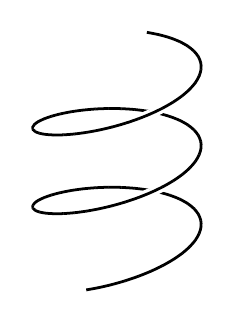
\begin{tikzpicture}[rubout/.style={/utils/exec=\tikzset{rubout/.cd,#1},
        decoration={show path construction,
        curveto code={
            \draw [white,line width=\pgfkeysvalueof{/tikz/rubout/line width}+2*\pgfkeysvalueof{/tikz/rubout/halo}]
            (\tikzinputsegmentfirst) .. controls
            (\tikzinputsegmentsupporta) and (\tikzinputsegmentsupportb)  ..(\tikzinputsegmentlast);
            \draw [line width=\pgfkeysvalueof{/tikz/rubout/line width},shorten <=-0.1pt,shorten >=-0.1pt] (\tikzinputsegmentfirst) .. controls
            (\tikzinputsegmentsupporta) and (\tikzinputsegmentsupportb) ..(\tikzinputsegmentlast);
        }}},rubout/.cd,line width/.initial=2pt,halo/.initial=0.5pt]
            \draw[rubout={line width=1pt,halo=1.2pt},decorate,
                domain=0:900,samples=101,smooth,variable=\t]
            plot({sin(\t)},\t/360,{cos(\t)});
        \end{tikzpicture}
        \caption{Intuitively, if we keep zooming in, we get a straight line on the spiral}
        \label{fig:spiral}
    \end{figure}
\end{tcolorbox}

In essence, an $n$-dimensional manifold ``looks like" $\mathbb{R}^n$ locally.

\subsection{Formal Definition of Manifolds}

The chief problem with the \hyperref[subsec:intuitive-manifolds]{intuitive introduction of manifolds} is that it depends
on having an ``ambient Euclidean space" in which our $n$-manifold lives. This introduces a great deal of extraneous
structure that is irrelevant to our purpose. Instead, we would like to view a manifold as a mathematical object in its
own right, not as a subset of some larger space. They key concept that makes this possible is that of a
\textit{topological space}.



\begin{Definition}{Continuous Mapping}{continuous-mapping}
    If $(M_1, d_1)$ and $(M_2, d_2)$ are metric spaces and $x$ is a point in $M_1$, a map $f: M_1 \rightarrow M_2$ is
    said to be \textbf{continous at $x$} if for any $\epsilon > 0$ there exists $\delta > 0$ such that
    $d_1(x, y) < \delta$ implies $d_2(f(x), f(y)) < \epsilon$ for all $y \in M_1$; and $f$ is \textbf{continuous} if it
    is continuous at every point of $M_1$\footnote{\href{https://trello.com/c/SI33o8fG}{Introduction to Topological Manifolds}, John M. Lee, 2nd, P.398}
\end{Definition}

\begin{Definition}{Image}{image}
    Let $f: X \rightarrow Y$ be a function. If $S \subset X$, the \textbf{image of $S$ under $f$}, denoted by $f(S)$, is
    the subset of $Y$ defined by\footnote{\href{https://trello.com/c/SI33o8fG}{Introduction to Topological Manifolds}, John M. Lee, 2nd, P.387}

    \begin{equation}
        f(S) = \{ y \subseteq Y: y = f(x) \text{ for some } x \in S \}
    \end{equation}
\end{Definition}

\begin{Definition}{Preimage}{preimage}
    If $T$ is a subset of $Y$, the \textbf{preimage of $T$ under $f$} (also called the \textbf{inverse image}) is the
    subset $f^{-1}(T) \subseteq X$ defined by\footnote{\href{https://trello.com/c/SI33o8fG}{Introduction to Topological Manifolds}, John M. Lee, 2nd, P.388}

    \begin{equation}
        f^{-1}(T) = \{ x \in X : f(x) \in T \}
    \end{equation}
\end{Definition}

\begin{Definition}{Open Subset}{open-subset}
    Let $M$ be a \hyperref[def:metrix-space]{metric space}

    \begin{itemize}
        \item For any $x \in M$ and $r > 0$, the \textbf{(open) ball of radios $r$ around $x$} is the set

              \begin{equation}
                  B_r(x) = {y \in M : d(y, x) < r}
              \end{equation}

              and the \textbf{closed ball of radios $r$ around $x$} is

              \begin{equation}
                  \overline{B}_r(x) = {y \in M : d(y, x) \le r}
              \end{equation}

        \item A subset $A \subseteq M$ is said to be an \textbf{open subset of $M$} if it contains an open ball around
              each of its points
        \item A subset $A \subseteq M$ is said to be a \textbf{closed subset of $M$} if
    \end{itemize}
\end{Definition}
